\documentclass[tikz,border=10pt]{standalone}
\usepackage[T1]{fontenc}
\usepackage{lmodern}
\usepackage{amsmath,amssymb}
\usetikzlibrary{arrows.meta,positioning}
\definecolor{ink}{HTML}{203044}
\definecolor{line}{HTML}{798899}
\definecolor{exact}{HTML}{EEF5F0}
\definecolor{approx}{HTML}{EEF3FA}
\begin{document}
\pagecolor{white}
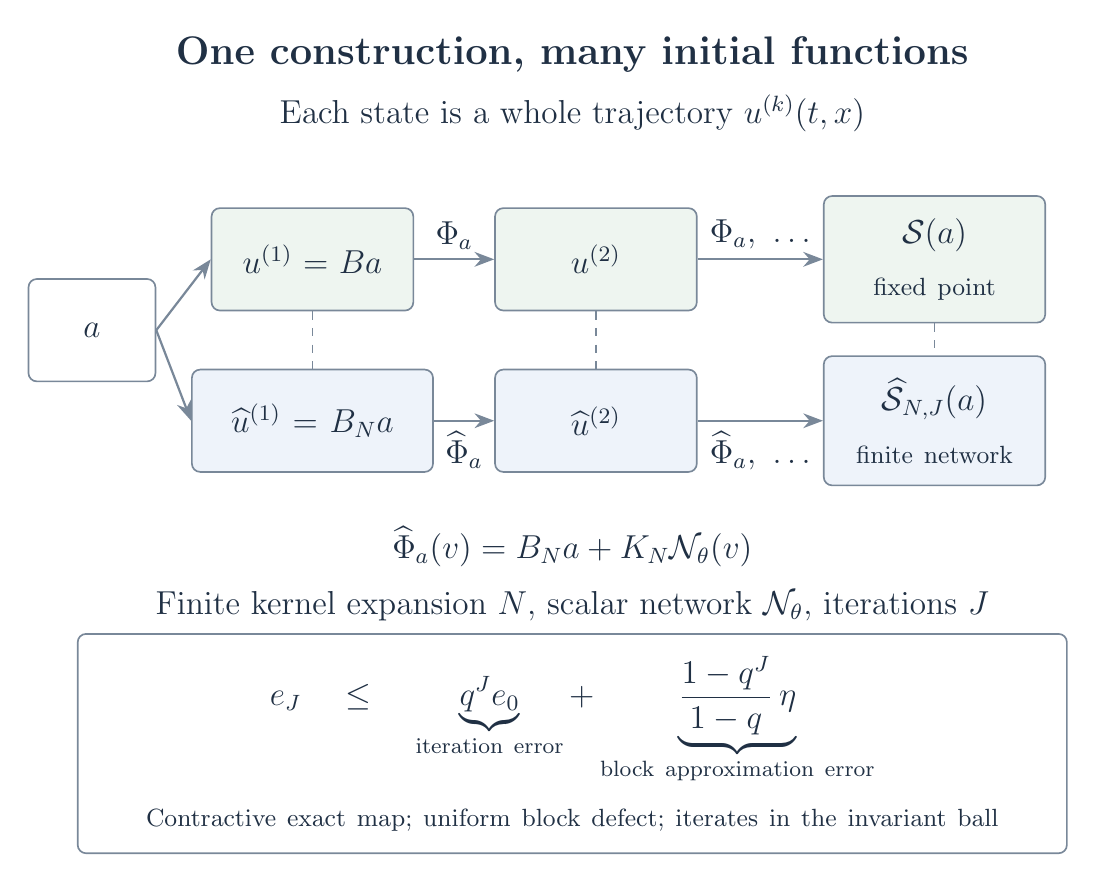
\begin{tikzpicture}[
  text=ink,
  box/.style={draw=line, line width=.6pt, rounded corners=3pt,
    align=center, inner sep=8pt, font=\large, minimum height=1.3cm},
  arrow/.style={-{Stealth[length=2.5mm]}, draw=line, line width=.8pt},
  compare/.style={dashed, draw=line, line width=.65pt},
  label/.style={font=\large, align=center}
]
  \node[font=\Large\bfseries] at (6.1,2.6) {One construction, many initial functions};
  \node[label] at (6.1,1.85)
    {Each state is a whole trajectory \(u^{(k)}(t,x)\)};

  \node[box, text width=1.05cm] (a) at (0,-.9) {\(a\)};
  \node[box, fill=exact, text width=2.0cm] (u1) at (2.8,0) {\(u^{(1)}=Ba\)};
  \node[box, fill=exact, text width=2.0cm] (u2) at (6.4,0) {\(u^{(2)}\)};
  \node[box, fill=exact, text width=2.25cm] (solution) at (10.7,0)
    {\(\mathcal S(a)\)\\[5pt]\small fixed point};
  \draw[arrow] (a.east) -- (u1.west);
  \draw[arrow] (u1.east) -- node[above, label] {\(\Phi_a\)} (u2.west);
  \draw[arrow] (u2.east) -- node[above, label] {\(\Phi_a,\ \ldots\)} (solution.west);

  \node[box, fill=approx, text width=2.5cm] (v1) at (2.8,-2.05)
    {\(\widehat u^{(1)}=B_Na\)};
  \node[box, fill=approx, text width=2.0cm] (v2) at (6.4,-2.05)
    {\(\widehat u^{(2)}\)};
  \node[box, fill=approx, text width=2.25cm] (operator) at (10.7,-2.05)
    {\(\widehat{\mathcal S}_{N,J}(a)\)\\[5pt]\small finite network};
  \draw[arrow] (a.east) -- (v1.west);
  \draw[arrow] (v1.east) -- node[below, label] {\(\widehat\Phi_a\)} (v2.west);
  \draw[arrow] (v2.east) -- node[below, label] {\(\widehat\Phi_a,\ \ldots\)} (operator.west);
  \draw[compare] (u1.south) -- (v1.north);
  \draw[compare] (u2.south) -- (v2.north);
  \draw[compare] (solution.south) -- (operator.north);

  \node[label] at (6.1,-3.65)
    {\(\widehat\Phi_a(v)=B_Na+K_N\mathcal N_\theta(v)\)};
  \node[label] at (6.1,-4.4)
    {Finite kernel expansion \(N\), scalar network \(\mathcal N_\theta\), iterations \(J\)};
  \node[box, text width=12.0cm, minimum height=1.65cm] at (6.1,-6.15)
    {\(\displaystyle
      e_J\ \le\
      \underbrace{q^J e_0}_{\text{iteration error}}
      +\underbrace{\frac{1-q^J}{1-q}\,\eta}_{\text{block approximation error}}
    \)\\[8pt]
    \small Contractive exact map; uniform block defect; iterates in the invariant ball};
\end{tikzpicture}
\end{document}
